\documentclass{article}

\usepackage[utf8]{inputenc} 
\usepackage{outlines}
\usepackage{amsmath}
\usepackage{cleveref}
\usepackage{siunitx}
\usepackage{multirow}
\usepackage{float}


\usepackage{natbib}
\bibliographystyle{abbrvnat}

\usepackage[margin=1in]{geometry}
\parskip 1.5ex % paragraph spacing

\usepackage{graphicx}
\graphicspath{./docs/Figures/}

%external references
\usepackage{xr}
\makeatletter
\newcommand*{\addFileDependency}[1]{% argument=file name and extension
  \typeout{(#1)}
  \@addtofilelist{#1}
  \IfFileExists{#1}{}{\typeout{No file #1.}}
}
\makeatother

\newcommand*{\myexternaldocument}[1]{%
    \externaldocument{#1}%
    \addFileDependency{#1.tex}%
    \addFileDependency{#1.aux}%
}

\myexternaldocument{./docs/Maintext/main}


\title{Supplementary Material for: \\ 
Variation in thermal sensitivity of ecological traits drives patterns of microbial community richness across temperature gradients }
\author{Tom Clegg, Samraat Pawar}
\date{January 2021}

\begin{document}

\maketitle

\renewcommand{\thepage}{S\arabic{page}} 
\renewcommand{\thesection}{S\arabic{section}}  
\renewcommand{\thetable}{S\arabic{table}}  
\renewcommand{\thefigure}{S\arabic{figure}} 
\renewcommand{\figurename}{Supplemental Figure} 
\renewcommand{\theequation}{S\arabic{equation}} 


\section{Mean-field approximation} \label{SI_Sec:Meanfield}
In this section we derive the mean-field approximation for equilibrium species' abundances in a microbial community, which then allows us to derive general conditions for a system to be feasible (all species to have a positive abundance at equilibrium).Broadly, the mean-field approximation considers the effect of species interactions in terms of their average effect on population abundances instead of individual effects of the pairwise interactions. We start by rewriting the species interactions term in the GLV (main text \cref{EQ:GLVM}) as:
\begin{equation} \label{EQ:mean_int} 
    \sum^N_{i \neq j} a_{ij} x_j = (N-1) \overline{a x} = (N-1) \bar{a} \bar{x} + (N-1) \text{cov}(a, x),
\end{equation}
where $\bar{\cdot}$ represents the average of that quantity over all $N$ species in the system. \Cref{EQ:mean_int} partitions the effects of interactions on the $i$th species into the average effect across the system, $\bar{a} \bar{x}$, and the covariance between heterospecific's biomass and the strength of interactions, $\text{cov}(a,x)$. The mean-field approximation assumes that this second term is negligible, which is equivalent to saying that any individual interaction between the focal species and another species population has little effect on that heterospecific's biomass. We also assume here that the system we consider is large ($N \gg 0$), meaning that the difference between the average biomass across the system and that of heterospecifics is small (as it is in the order $N^{-1}$) and can thus be ignored. Finally we assume that intraspecific interactions are constant across populations with value of $1$. Combining \cref{EQ:GLVM,EQ:mean_int} we can then express population dynamics in terms the average interaction strength, giving the full mean-field model:

\begin{equation} \label{EQ:MF}
    \frac{1}{x_i} \frac{dx_i}{dt} \approx r_i - x_i - (N-1)\bar{a}(T)\bar{x}.
\end{equation}

Next, we obtain an expression for equilibrium by setting \cref{EQ:MF} equal to zero and solving for $x_i$ giving:

\begin{equation} \label{EQ:MF_partial}
    x_i^* = r_i(T) - (N-1)\bar{a}(T)\bar{x}^*.
\end{equation}
 
 Then, taking the average across the $N$ populations and rearranging we obtain an expression for the average biomass in the community:
 
 \begin{equation*}
     \bar{x}^* = \frac{\bar{r}(T)}{1 + (N-1)\bar{a}(T)},
 \end{equation*}
 
 which we can then substitute into \cref{EQ:MF_partial} to get equilibrium biomass:
 
 \begin{equation*}
     x_i^* = r_i(T) - \bar{r}(T) \frac{(N-1) \bar{a}}{1 + (N-1) \bar{a}}.
 \end{equation*}

Next we can see that in the case of no interspecific interactions ($\bar{a} = 0$) \cref{EQ:MF_partial} gives the carrying capacity, the biomass a species would reach if grown in isolation $x_i^* = r_i(T) = K_i(T)$ which gives us the final mean-field biomass expression:

\begin{equation*}
    x_i^* = K_i(T) - \bar{K(T)}\frac{(N-1)\bar{a}}{1 + (N-1)\bar{a}}
\end{equation*}

which is equivalent to \cref{EQ:MF_equi} in the main text.

\section{Derivation of thermal response distributions} \label{SI_Sec:TPC_dist}

In order to derive the distribution of some trait value $B(T)$ from the distribution of its thermal sensitivity parameters $B_0$s and $E$s we start with the Boltzmann-Arrhenius as detailed in the main text:

\begin{equation*}
    B(T) = B_0 e^{-\frac{E}{k} \left(\frac{1}{kT} - \frac{1}{k T_{ref} }\right)},
\end{equation*}
 
which taking the natural log gives:

\begin{equation} \label{EQ:LogBoltzmann}
    \log(B(T)) = \log(B_0) - \frac{E}{k} \left(\frac{1}{kT} - \frac{1}{kT_{ref}} \right).
\end{equation}
 
Next we assume that both $\log(B_0)$ and $E$ are normally distributed such that:
\begin{align*}
    \log(B_0) \sim \mathcal{N}(\mu_{B_0}, \sigma_{B_0}), \\
    \\
    log(E) \sim \mathcal{N}(\mu_E, \sigma_{E}),
\end{align*}

where $\mu_{B_0}$ and $\mu_E$ are the mean and $\sigma_{B_0}^2$ and $\sigma_{E}^2$ are the variances of the normalisation constant and thermal sensitivity respectively. This assumption is backed for $B_0$ by the distributions of actual values observed in our meta-analysis of bacterial population traits. Whilst distributions of $E$ tend to be more skewed in reality (as seen in both our data and previous work (REF)) we use the normal distribution here as it remains a good approximation, and a convenient way to account for variance in thermal sensitivity values. Now, considering \cref{EQ:LogBoltzmann} as a linear function of two normally distributed variables we can see that $\log(B(T))$ will itself be normally distributed as:

\begin{align*} 
    \log(B(T)) \sim \mathcal{N}\left(\mu_{B}(T) , \sigma_{B}^2(T) \right) 
    \quad \text{where} \quad
    \begin{array}{cc}
        \mu_B(T) &= \mu_{B_0} - \mu_{E} \left(\frac{1}{kT} - \frac{1}{k T_{ref} }\right)  \\
        \sigma_{B}(T)^2 &= \sigma_{B_0}^2 + \sigma_{E}^2 \left(\frac{1}{kT} - \frac{1}{k T_{ref} }\right)^2
    \end{array}
\end{align*}

which is the same as \cref{EQ:Boltz_dist} in the maintext. 

\subsubsection{Distribution of $\kappa$ and $\bar{a}$}

Next we apply the expression for the distribution of a trait across populations at a given temperature to the distribution of $\kappa$ and the value of $\bar{a}$ which determines feasibility in \cref{EQ:P_feas}. 

We start with $\kappa$ by recalling that as the relative carrying capacity $\kappa$ is defined as:

\begin{equation*}
    \kappa(T) = \frac{K(T)}{\bar{K}(T)}.
\end{equation*}

Assuming that $K$'s temperature dependence follows an Arrhenius-type form and that its thermal sensitivity parameters are distributed as described in \cref{EQ:Boltz_dist} we can see that:

\begin{equation*}
    \bar{K}(T) = e^{\mu_K(T) + \frac{\sigma_K(T)^2}{2}}
\end{equation*}

which applying to the equation above and taking the natural log gives:

\begin{equation*}
    \log(\kappa(T)) = \log(K(T)) - \mu_K(T) - \frac{\sigma_K(T)^2}{2}.
\end{equation*}

Thus, $\log(\kappa)$ is normally distributed as:

\begin{equation*}
    \log(\kappa(T)) \sim \mathcal{N}\left(-\frac{\sigma_K(T)^2}{2},\sigma_K(T)\right).
\end{equation*}

The thermal dependence of $\bar{a}$ is obtained by by simply considering $a(T)$ which, assuming it follows a Arrhenius-type response with temperature and again its thermal sensitivity parameters are distributed as described in \cref{EQ:Boltz_dist} has an average given by:

\begin{equation*}
    \bar{a}(T) = e^{\mu_a(T) + \frac{\sigma_a(T)^2}{2}}.
\end{equation*}

\newpage

\section*{Supplementary Figures}

\begin{figure}[H]
    \centering
    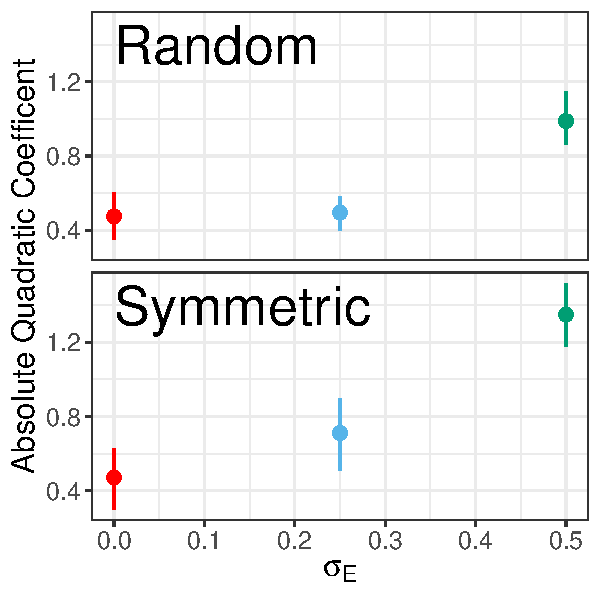
\includegraphics[width = 0.4\textwidth]{docs/Figures/Fig_QuadCoef.pdf}
    \caption{\textbf{The degree of the unimodality in the richness-temperature relationship increases with $\sigma_E$} The absolute size of the quadratic coefficient from polynomial fits of final richness vs temperature increases with increasing variation in both the random and symmetric mixed interaction cases. Each point represents the absolute mean estimate of the quadratic coefficient for a given level of variation (moving left to right) and interaction scenario. Ranges around each point represent the bootstrapped $2.5\%$ and $97.5\%$ confidence intervals.}
    \label{SIFig:quad_coeff}
\end{figure}

\end{document}